%This chapter introduces the SM and the important interactions
%Then top physics is introduced talking about the decay
%tW and tt bar and their crosssections
%What is NLO and LO when are the diagrams similar
%Motivate the difficulties

\chapter{Theoretical basics}

In this chapter the Standard Model of Particle Physics, or Standard Model, with its elementary particles and interactions is introduced.
Furthermore, the analysis in this thesis is motivated and the underlying problems are outlined. For this reason a brief introduction to the theory of particle production and decay is given.


\section{The Standard Model of Particle Physics}
\label{sec:sm}

Originally, created in an attempt to unify the electromagnetic, weak, and strong force under one theory, the Standard Model of particle physics represents the status quo in this field summarizing the elementary particles and their interactions.
The model is a gauge quantum field theory and its internal symmetry is the unitary product group $SU(3) \times SU(2) \times U(1)$ in which the interactions are represented by particles named gauge bosons.
Figure \ref{fig:sm} shows the Standard Model particles and their central properties which will be introduced in this chapter starting with the interactions and their mediators followed by a summary of the particles and lastly a section on the top-quark in addition to its properties directly relevant for the research in this thesis.

Although failing to answer open questions like the origin of dark matter or neutrino oscillations, the Standard Model has proven to be a powerful model being very successful in providing experimental predictions for decades.

\begin{figure}
	\centering
	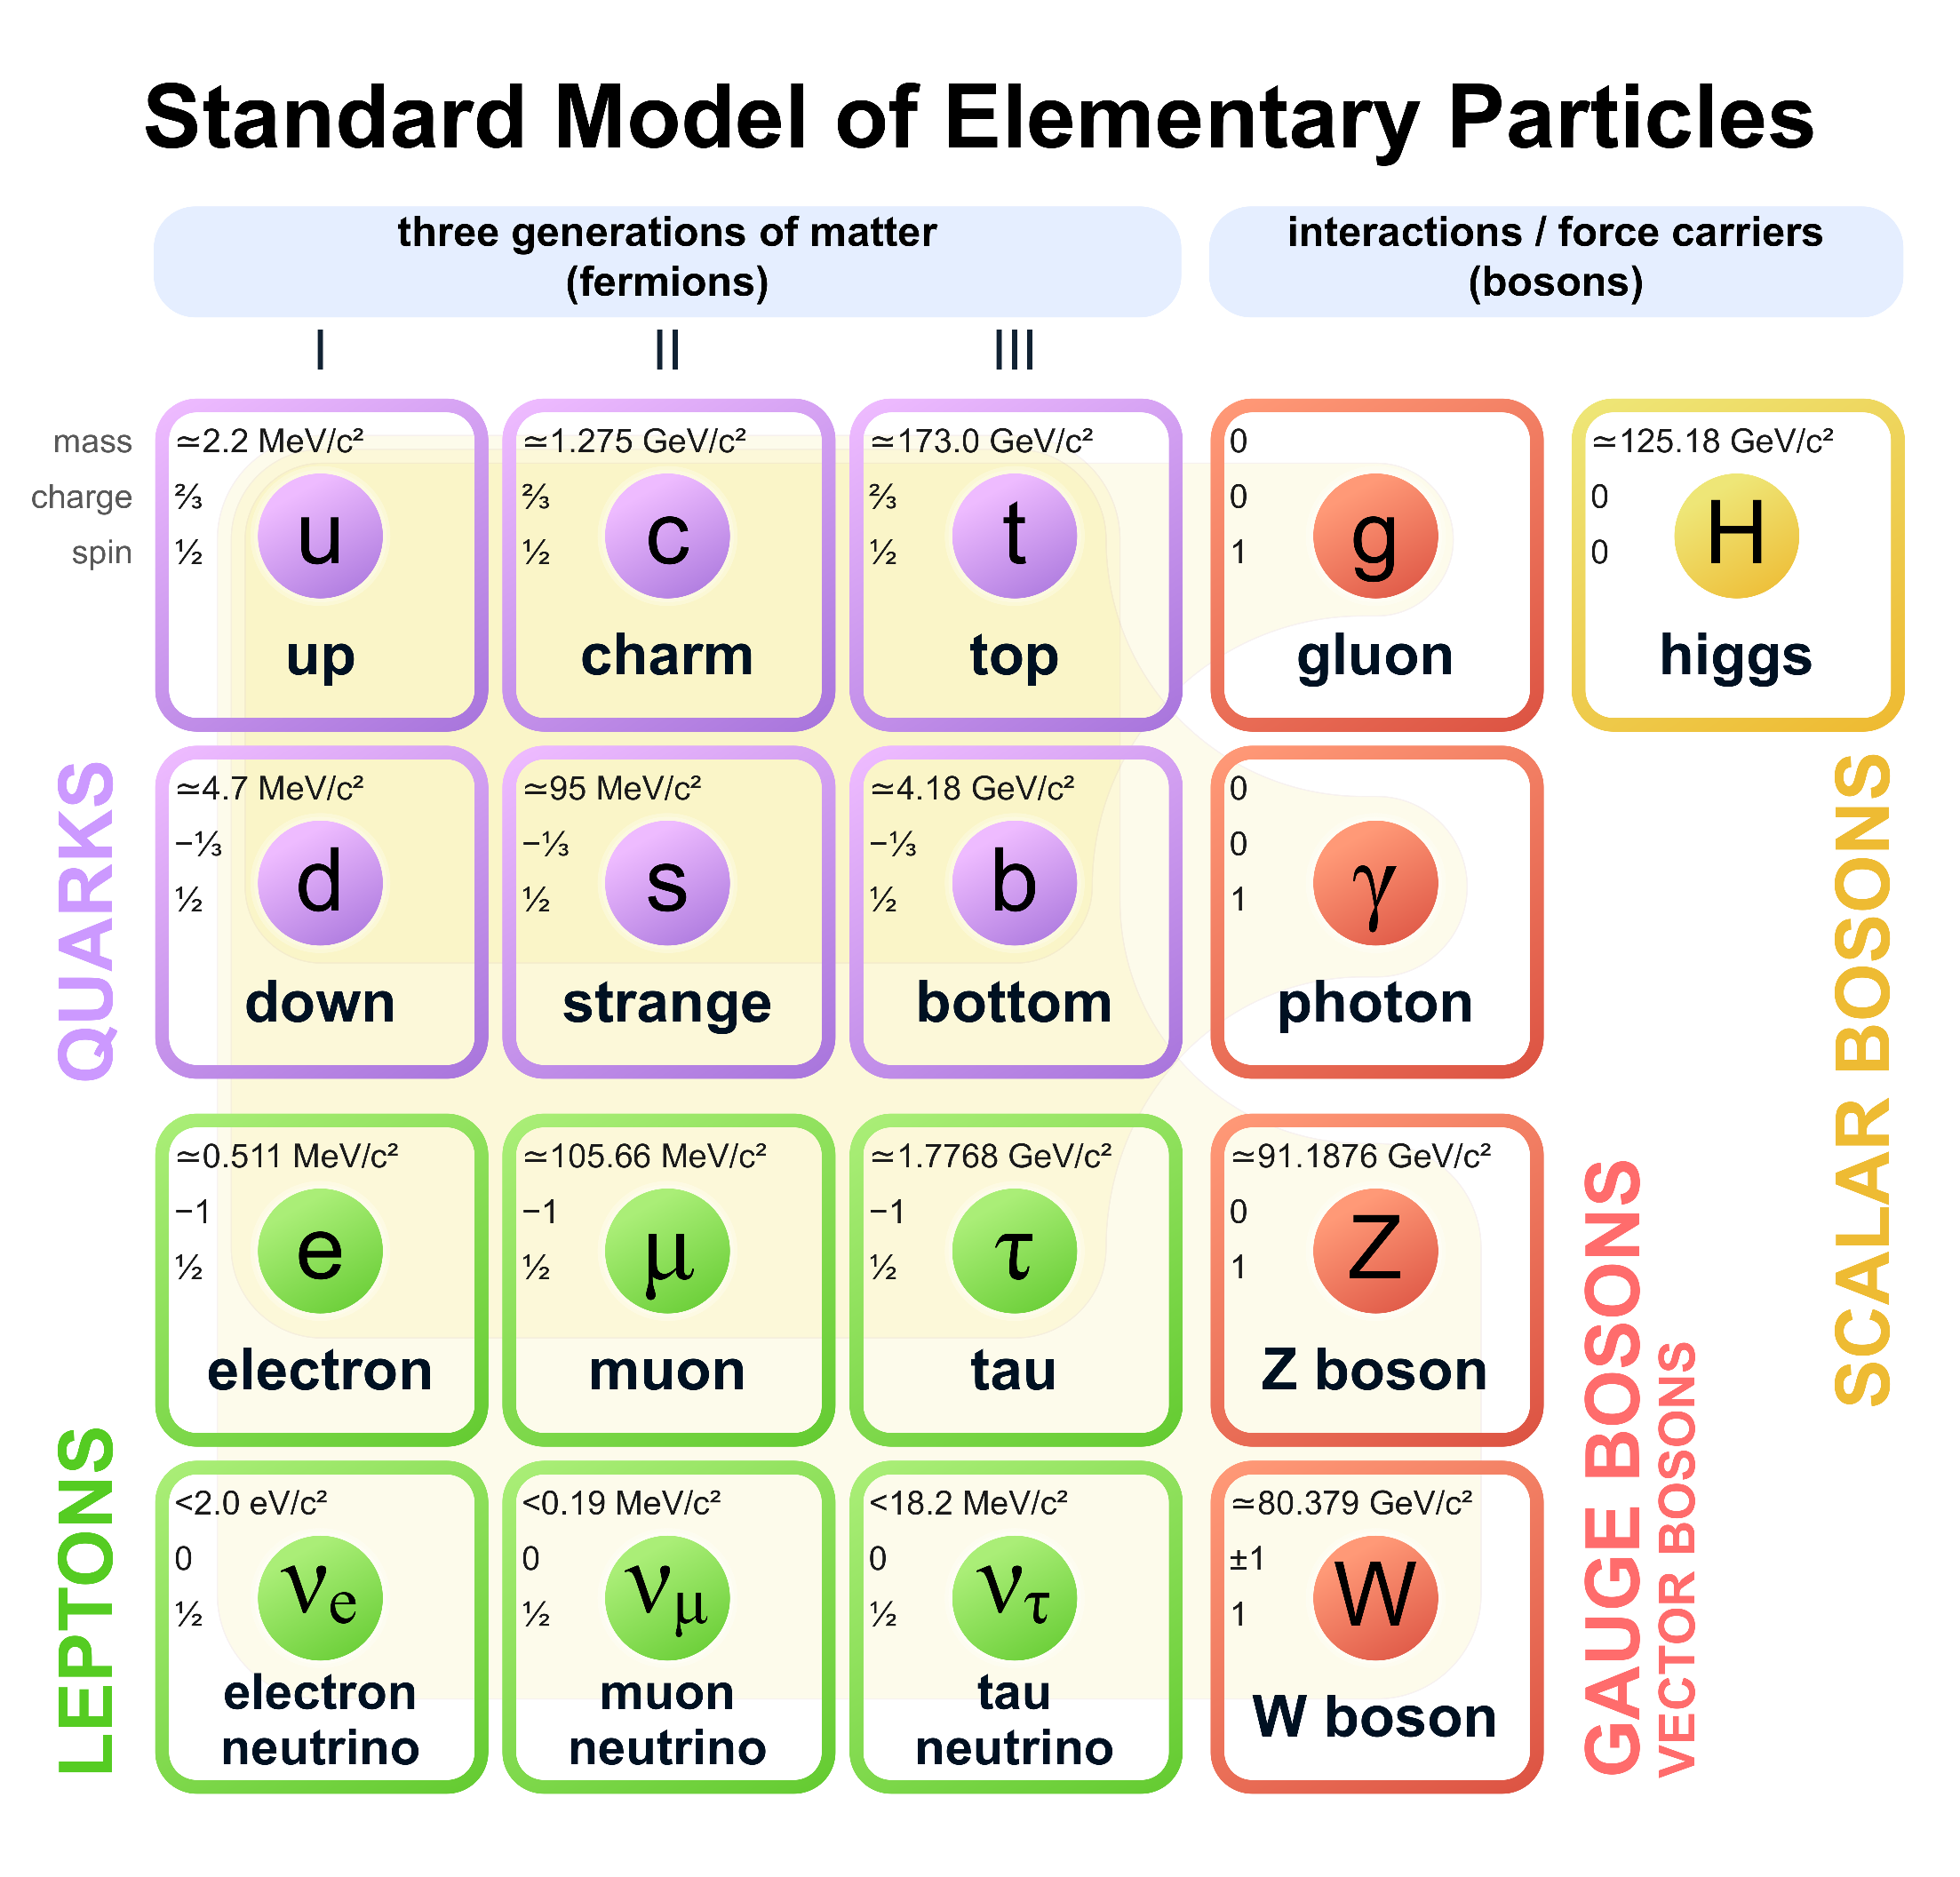
\includegraphics[width=0.8\textwidth]{figures_SM/standard_model.eps}
	\caption[Standard Model of Particle Physics]{Summary table of the Standard Model particles and their properties. The matter particles, quarks in purple and leptons in green, and the force carriers in red are shown. In addition, the Higgs, in yellow, is included as the latest addition to the model.  The sketch~\cite{standard_model} was updated to PDG 2018 data~\cite{PDG}}
	\label{fig:sm}
\end{figure}



\subsection{Force carrier particles}

There are three interactions represented in the Standard Model: the electromagnetic interaction, the weak interaction, and the strong interaction. Each is represented by an integer-spin particle, called \emph{mediator boson}. Gravity is usually not included in this model as it is negligible at this scale. 

The electromagnetic force is described by the theory of quantum electrodynamics. Its mediator is the photon, a massless particle that couples to the electric charge.
The weak force, most commonly known as the interaction responsible for the $\beta$-decay, couples to the weak charge; which is an intrinsic property of all fermions. Its mediators are the \PZ- and the two opposite-charged \PW-Bosons.
The electromagnetic and the weak force can be unified as the electroweak interaction forming a $SU(2) \times U(1)$ symmetry.
One aspect of the weak force is that it allows for quark-flavour change via an interaction with a \PW-boson. The probability of this flavour change is represented by the Cabibbo-Kobayashi-Maskawa matrix, CKM matrix, which is described in detail in the PDG~\cite{PDG}.

The strong force is responsible for the binding of quarks in the nucleon, the protons and neutrons. It is mediated by the \num{8} differently flavoured gluons. It only couples to particles with colour charge and is represented by the $SU(3)$ symmetry term in the Standard Model.

As already stated the gravitational force is not included in the Standard Model as its coupling strength at the scale is only of the order \num{10E-37}. Although it is not a mediator, the Higgs boson was included in the Standard Model after its discovery in 2012. It is the particle associated to the mechanism which gives all other particles mass.

\subsection{Matter particles}

The non-mediator particles in the model are called \emph{fermions}, which are half-integer spin. They can be broadly classified into three generations of leptons and quarks

The first generation of particles forms the most common form of matter. The electron, the electron-neutrino, and the up- and down-quark, which are the main constituents of the proton and neutron.
In the higher generations the defining quantum numbers stay the same while the mass of the particles increases.
The quarks that share the properties of the up-quark are called up-type quarks, and they are the charm- and top-quarks. In contrast, there are down-type quarks: the strange- and bottom-quarks. Bound quark states are called hadrons.
Moreover, there is an antiparticle for each particle with all quantum numbers reversed.

The neutrinos interact only via the weak interaction. There is one neutrino for each lepton-family.
The non-neutrino leptons are the electron, \Pelectron,the muon, \Pmu , and the tauon, \Ptau, in order of increasing mass. They have an intrinsic electric charge which allows them to interact electromagnetically.
Furthermore, the six quark flavours are up and down, strange and charm, bottom and top.
The quarks are the only particles interacting with all three forces. They carry not only a weak and an electric charge but also colour charge enabling them to interact with gluons.

\section{Top-quark physics}


The most essential aspects of particle interactions, underlying the events of interest of this work, are the production and decay processes of the top-quark. This section introduces the main properties of the top-quark. 
The top-quark, being the third generation up-type quark, is special because its mass exceeds the masses of the other quarks by orders of magnitude. Its mass is about \SI{173}{\GeVovercsq} which is higher than the masses of the weak mediators. 
It has a lifetime of $\mysim$ \SI{5E-25}{\second} which is smaller than the typical hadronisation time, meaning that the top-quark forms no bound states with other quarks and instead decays.
These essential properties of the heaviest quark lead to some interesting aspects and motivate one to research its properties.

To describe the production and decay of the top-quark Feynman-diagrams will be used. These diagrams are used to present the process and the underlying math. The time-axis is defined as the positive x-axis. Fermions are depicted by a solig line with an arrow; for particles it points with time and for antiparticles against it. Gluons are represented by curly the other bosons by wavy lines. Alternatively the mediators of the weak force are sometimes depicted using dashed lines.
In addition diagrams may be labeled with an order. The lowest order diagram is the \emph{leading order} process, LO. To achieve a higher precision corrections are applied. One then speaks of \emph{next-to-leading order}, NLO, where the next-to can added iteratively for even higher order corrections.


\subsection{Top-quark production}

Most commonly top-quarks are created via the strong force in a top- anti-top-quark final state. Both gluon-gluon fusion and quark-antiquark-annihilation are possible production processes. Figure~\ref{fig:ttpairLO} shows the processes at LO.
%
\begin{figure}[htbp]
  \begin{subfigure}[b]{0.3\textwidth}
  	\centering
    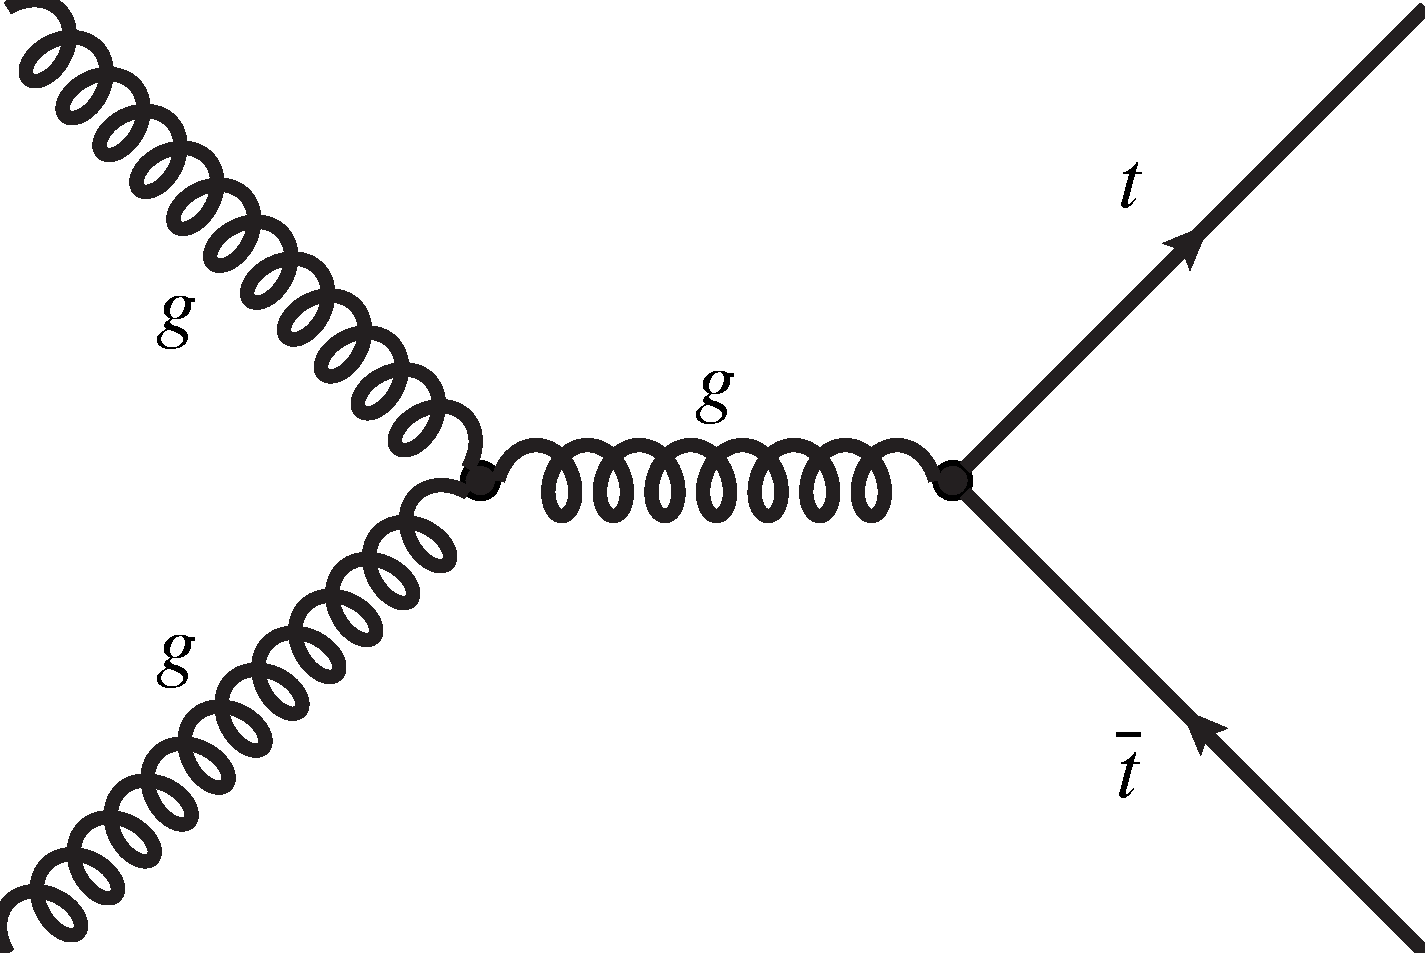
\includegraphics[height=3.5cm]{ttbar_ttbar_1-BW}
%    \caption{Picture 1}
%    \label{fig:1}
  \end{subfigure}
  \quad
  \begin{subfigure}[b]{0.3\textwidth}
  	\centering
    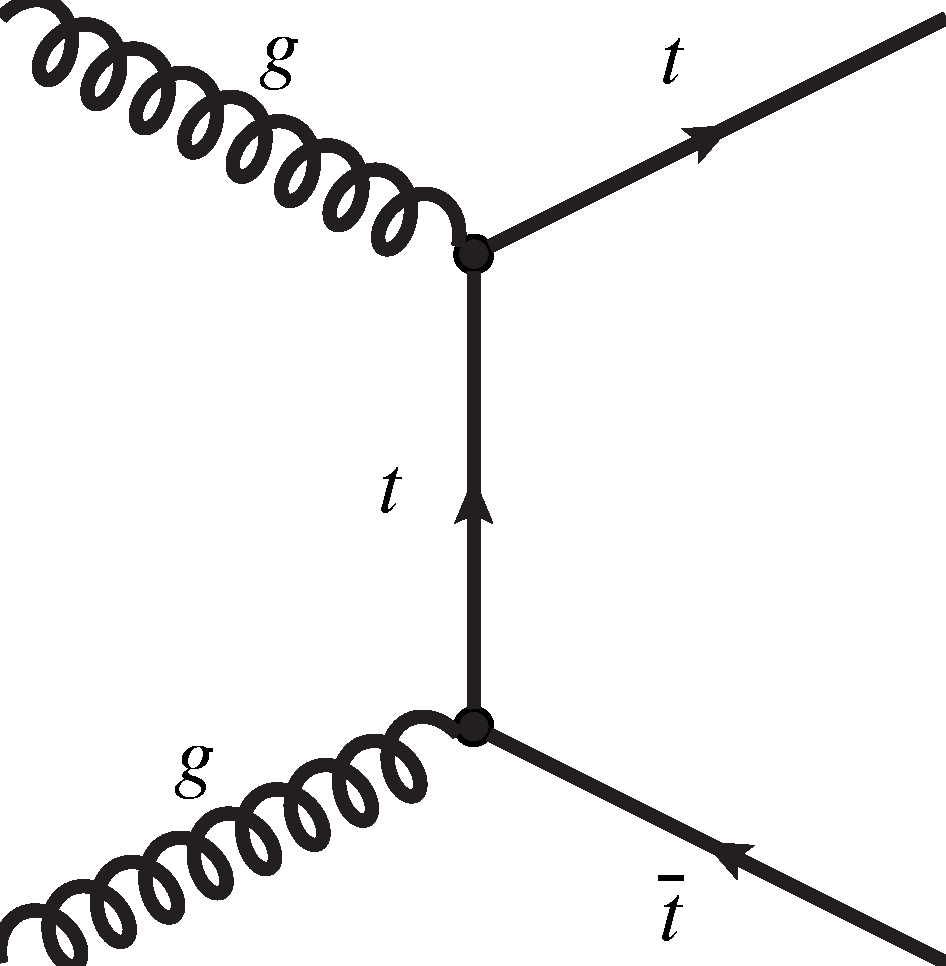
\includegraphics[height=3.5cm]{ttbar_ttbar_2-BW}
%    \caption{Picture 2}
%    \label{fig:2}
  \end{subfigure}
  \quad
  \begin{subfigure}[b]{0.3\textwidth}
  	\centering
    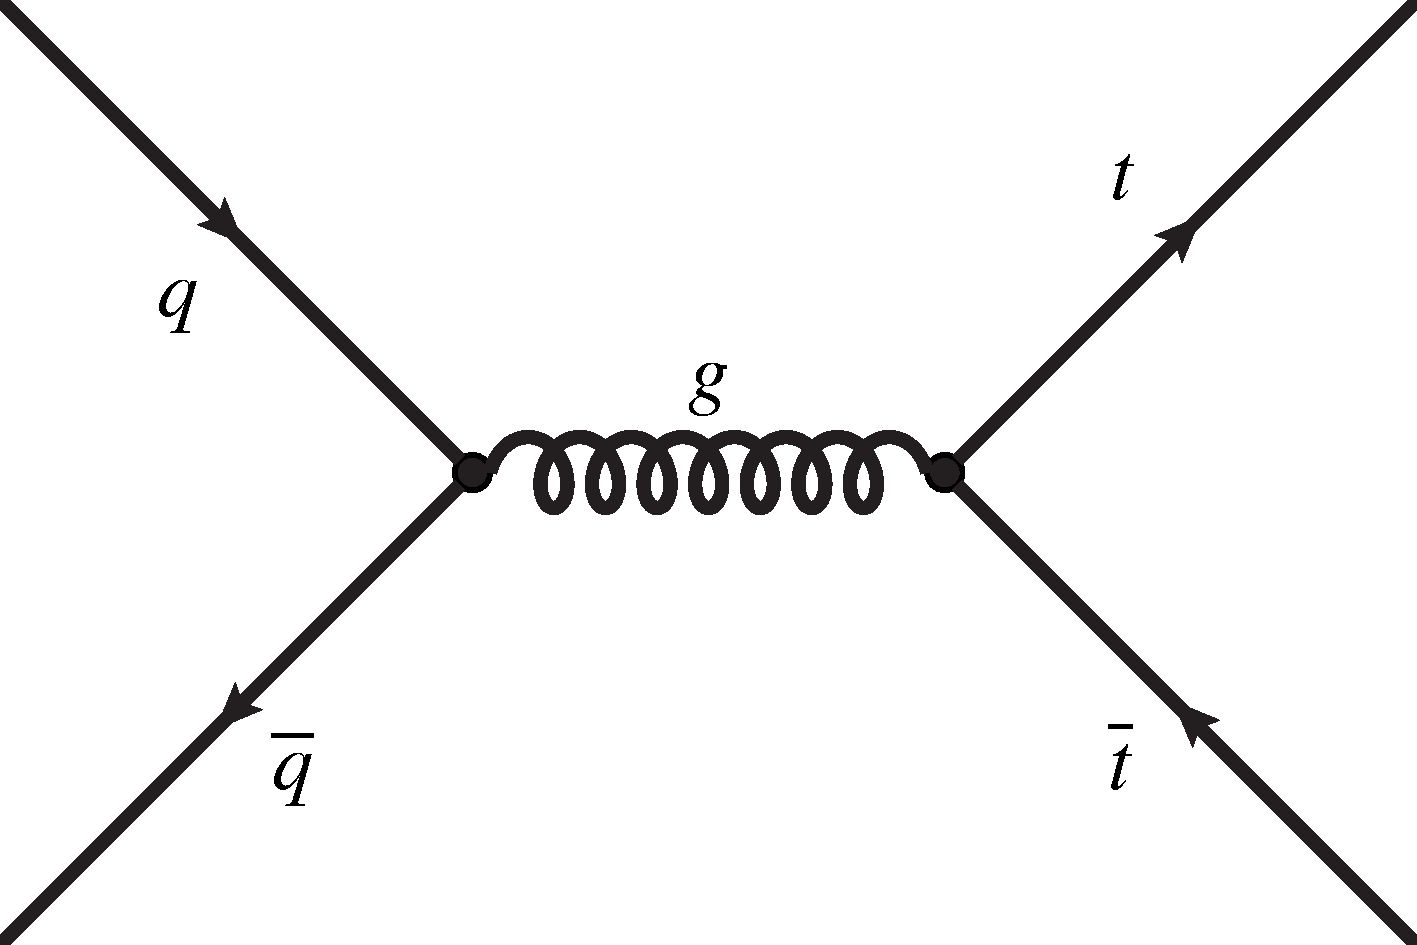
\includegraphics[height=3.5cm]{ttbar_ttbar_3-BW}
%    \caption{Picture 2}
%    \label{fig:2}
  \end{subfigure} 
  \caption[\ttbar pair production feynman diagrams at LO]{\ttbar pair production feynman diagrams at LO.}
  \label{fig:ttpairLO}
\end{figure}
%
Additionally, top-quarks can be produced as single top-quarks via the electroweak interaction. The dominant process is the production through the interaction of a bottom-quark and a \PW-boson shown in figure~\ref{fig:singletop:virtualWt}. Also possible but the least common is the s-channel involving a virtual \PW-boson displayed in figure~\ref{fig:singletop:virtualWs}. Finally the channel of interest for this work is the \tW-channel diagrammed in figure~\ref{fig:singletop:tW}.
The probability for a production to occur is denoted using the \emph{cross-section} of the process.

\subsection{Top-quark decay}

The top-quark almost exclusively decays into a W-boson and a bottom-quark. The \PW can subsequently decay leptonically, in a lepton-neutrino pair, or hadronically, in a quark-antiquark pair.
The channel of interest for this work is the \tW-channel which is diagrammed in figure~\ref{fig:singletop:tW}. The mode in which both \PW-bosons decay leptonically is investigated.
The analysis is described in greater detail in the following subsection.


\subsection{The \tW channel}
\label{sec:tw}

Finally the channel of interest for this work is the \tW-channel diagrammed in figure~\ref{fig:singletop:tW}.
Its final state only differs from the \ttbar-final state by one missing bottom-quark. This makes the \ttbar channel the dominant background for the \tW-signal.
The separation gets especially complicated because the cross-section of \tW is about \num{10} smaller than the \ttbar cross-section. The cross-sections for the channels are listed below:

\begin{align}
\sigma_{\tW} \mysim \SI{71.7}{\pb}\\
\sigma_{\ttbar} \mysim \SI{832}{\pb}.
\end{align}

Figure~\ref{fig:tw-decay} shows the final state of the \tW decay with both \PW-bosons decaying leptonically at LO. For that reason, the channel is named dilepton channel.
At NLO a gluon splitting can result into a further bottom-quark in the final state. Figure~\ref{fig:nlo} shows the \ttbar final state in comparison to the NLO final state of the \tW-channel. In the final state these channels are not distinguishable, {i.e.}, they interfere. These diagrams will be referred to as doubly resonant, in contrast to the singly resonant diagrams such as diagrammed in figure~\ref{fig:ttpairLO}.
Given that the \ttbar-cross-section is \num{10} orders larger than the \tW-cross-section this gives rise to an NLO correction exceeding the actual LO cross-section. This results in the \tW-channel not being well-defined at NLO.
To allow treating \tW as a separate process a workaround has to be used. There are two possible schemes for handling the interference in the calculation of the cross-section:

\begin{description}
\item[Diagram Removal (DR)] removes all diagrams containing a second top-quark propagator that can be on-shell. It is used for the production of the nominal sample in this work.
\item[Diagram Subtration (DS)] only the \ttbar contribution is canceled when the top-quark is on-shell. This scheme is used for the systematics sample.
\end{description}

For more information on the schemes and their motivation see section~\ref{sec:systmc},

\begin{figure}[htbp]
  \begin{subfigure}[b]{0.3\textwidth}
  	\centering
    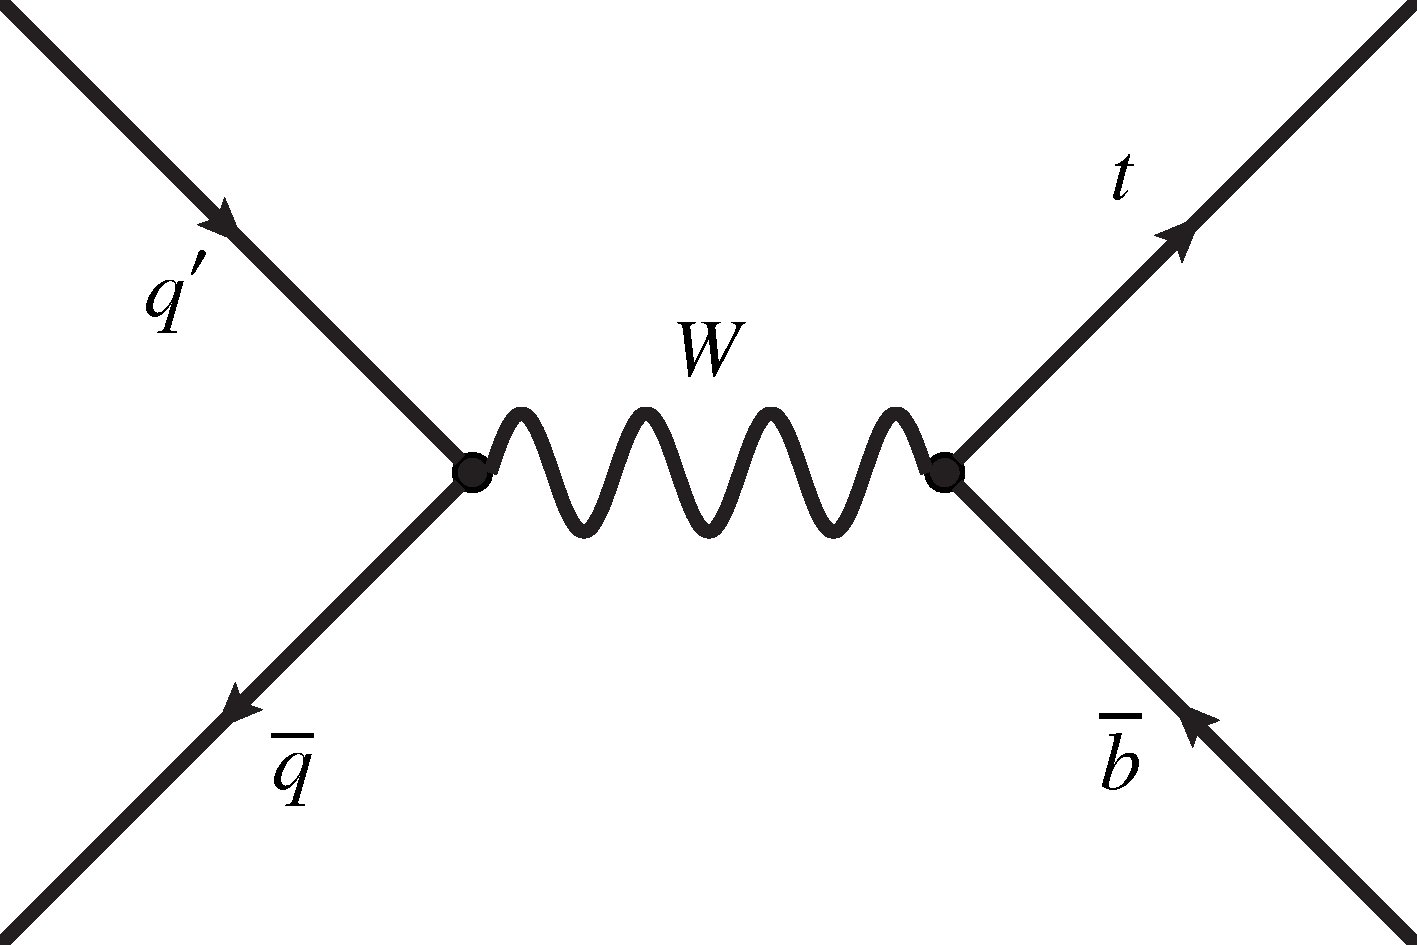
\includegraphics[height=3.5cm]{s-channel}
    \caption{}
    \label{fig:singletop:virtualWt}
  \end{subfigure}
  \quad
  \begin{subfigure}[b]{0.3\textwidth}
  	\centering
    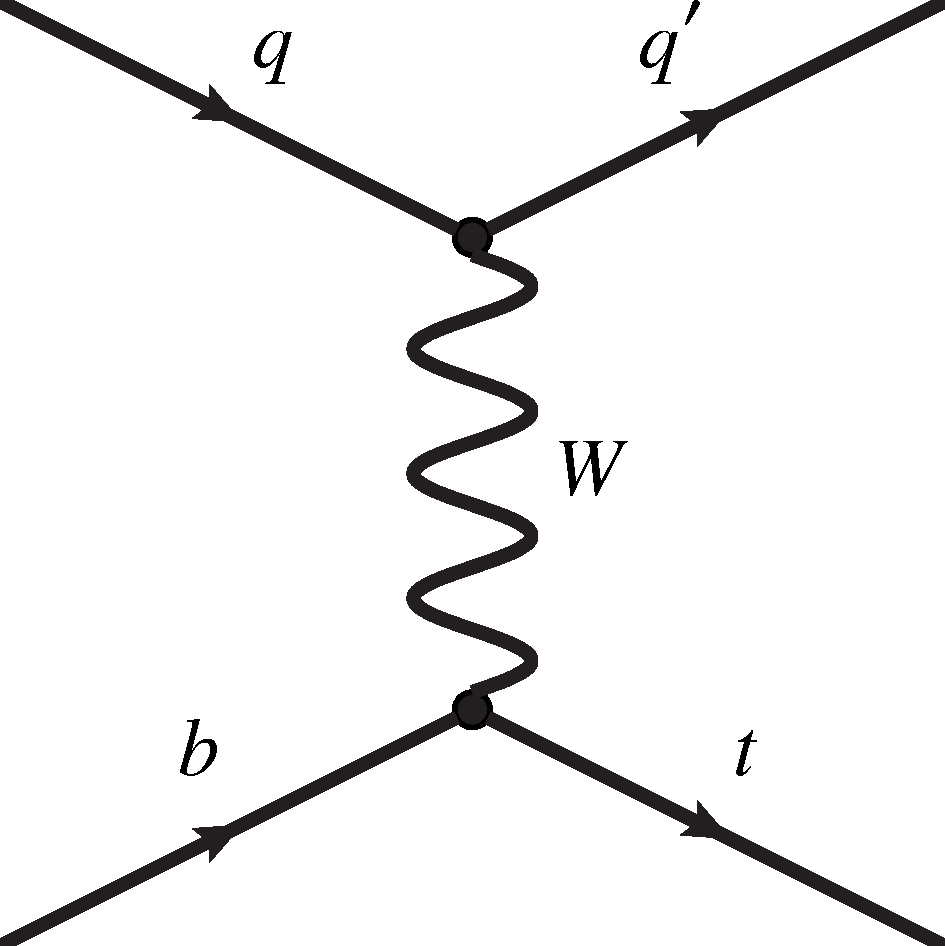
\includegraphics[height=3.5cm]{t-channel}
    \caption{}
    \label{fig:singletop:virtualWs}
  \end{subfigure}
  \quad
  \begin{subfigure}[b]{0.3\textwidth}
  	\centering
    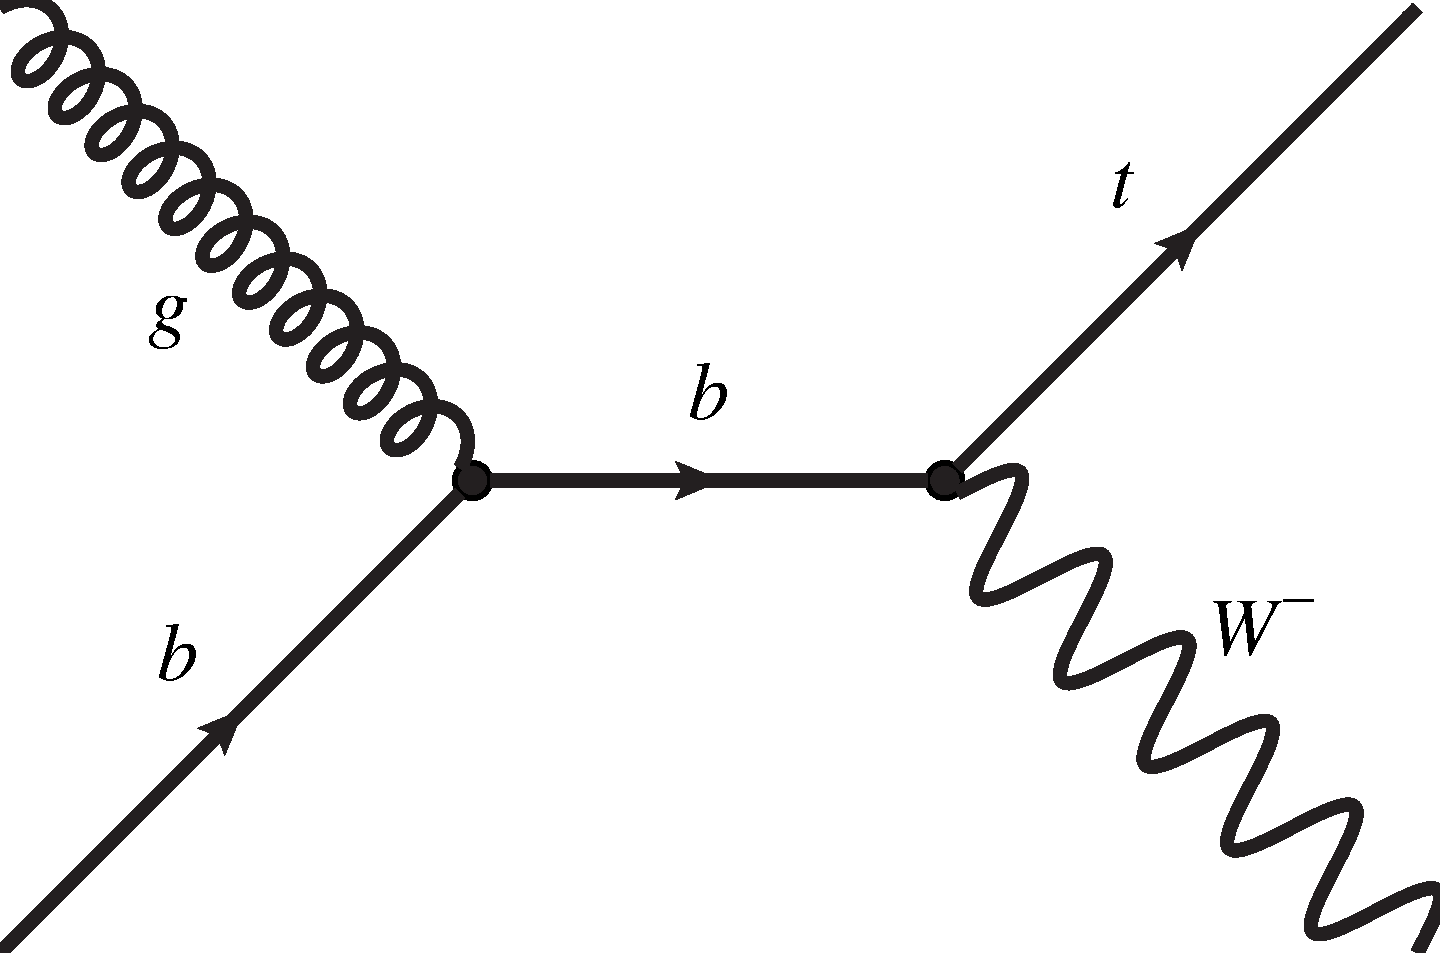
\includegraphics[height=3.5cm]{tW_channel}
    \caption{}
	\label{fig:singletop:tW}
  \end{subfigure} 
  \caption[Single-top-production diagrams]{Single-top-production diagrams: s-channel~\subref{fig:singletop:virtualWs}, t-channel~\subref{fig:singletop:virtualWt}, \tW-channel~\subref{fig:singletop:tW}}
  \label{fig:singletop}
\end{figure}


\begin{figure}[htbp]
	\centering
	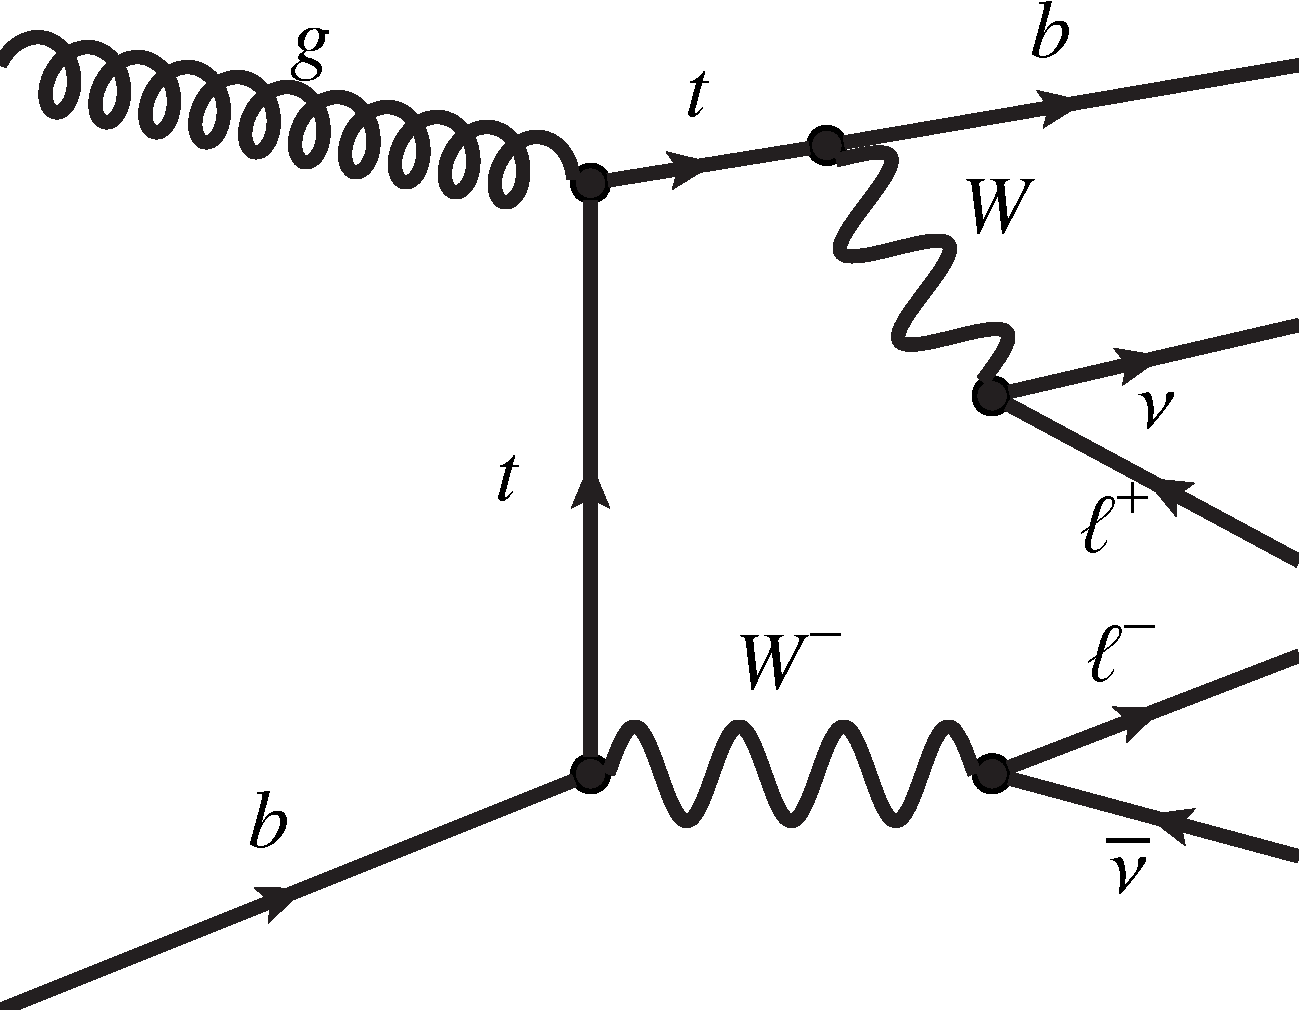
\includegraphics[width=0.8\textwidth]{tW-decay}
	\caption[Final state of a \tW decay]{Final state of a \tW decay. Both \PW-bosons decay leptonically, {i.e.}, in a lepton and the respective neutrino.}
	\label{fig:tw-decay}
\end{figure}

\begin{figure}[htbp]
    \centering
    \begin{subfigure}[b]{0.44\textwidth}
        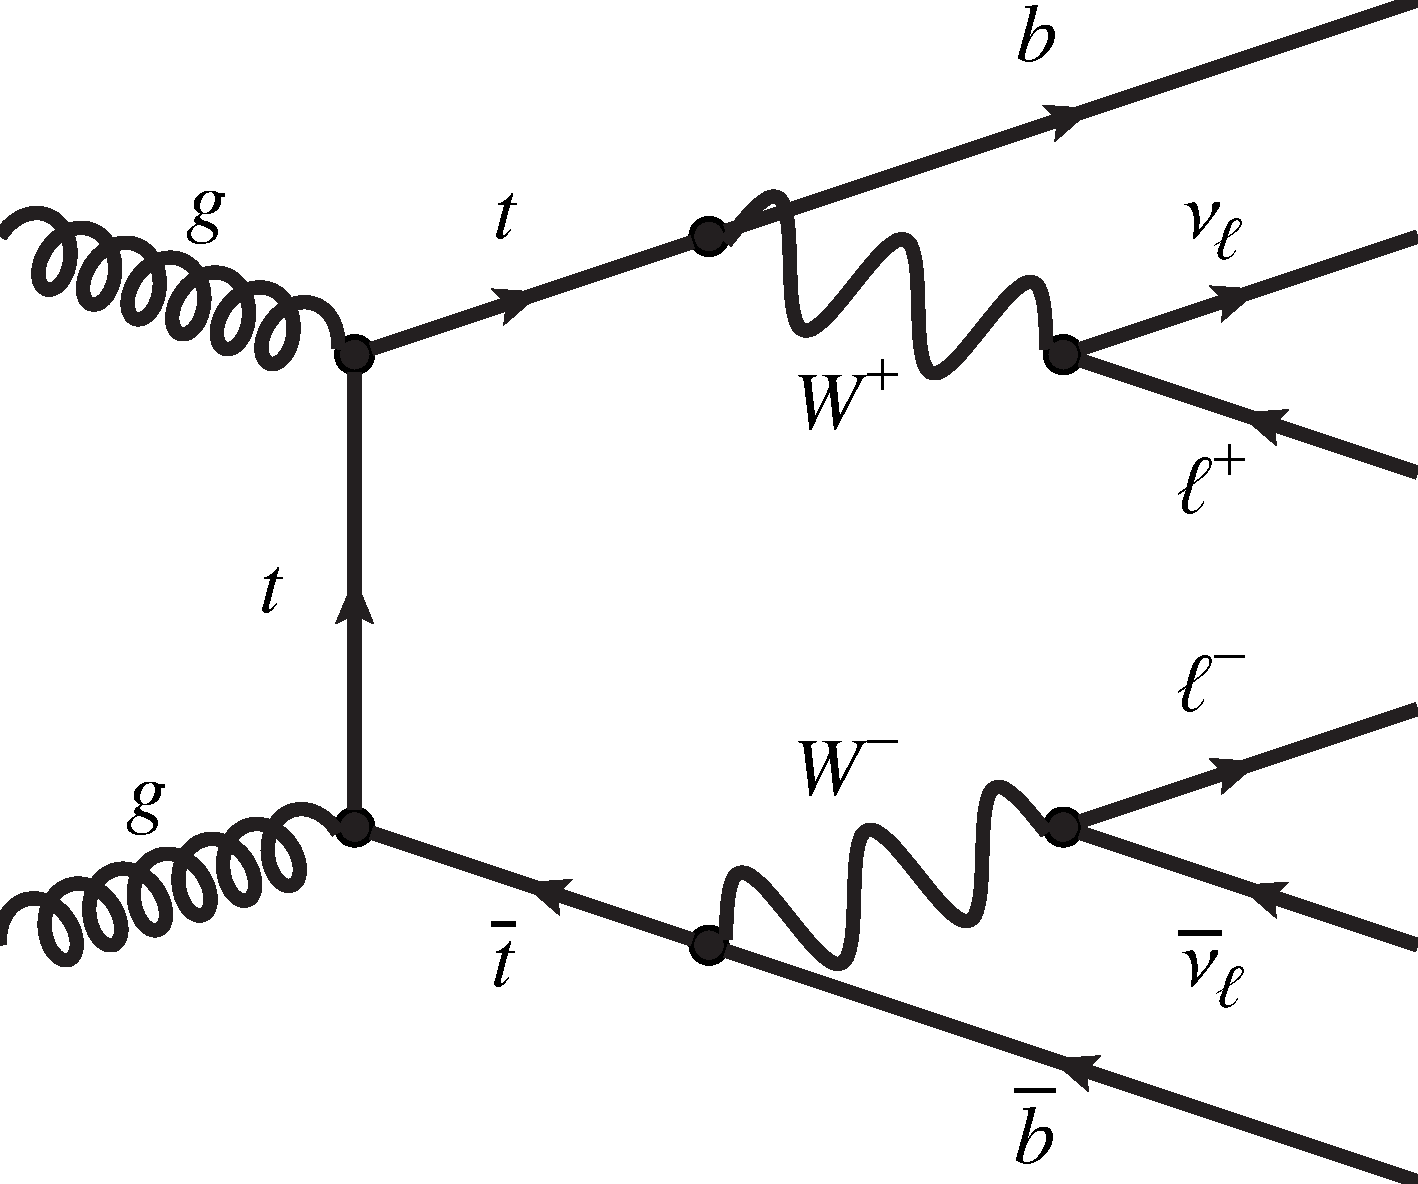
\includegraphics[width=\textwidth]{ttbar-decay}
        \caption{}
        \label{fig:nlo:ttbar}
    \end{subfigure}
\quad
    \begin{subfigure}[b]{0.44\textwidth}
        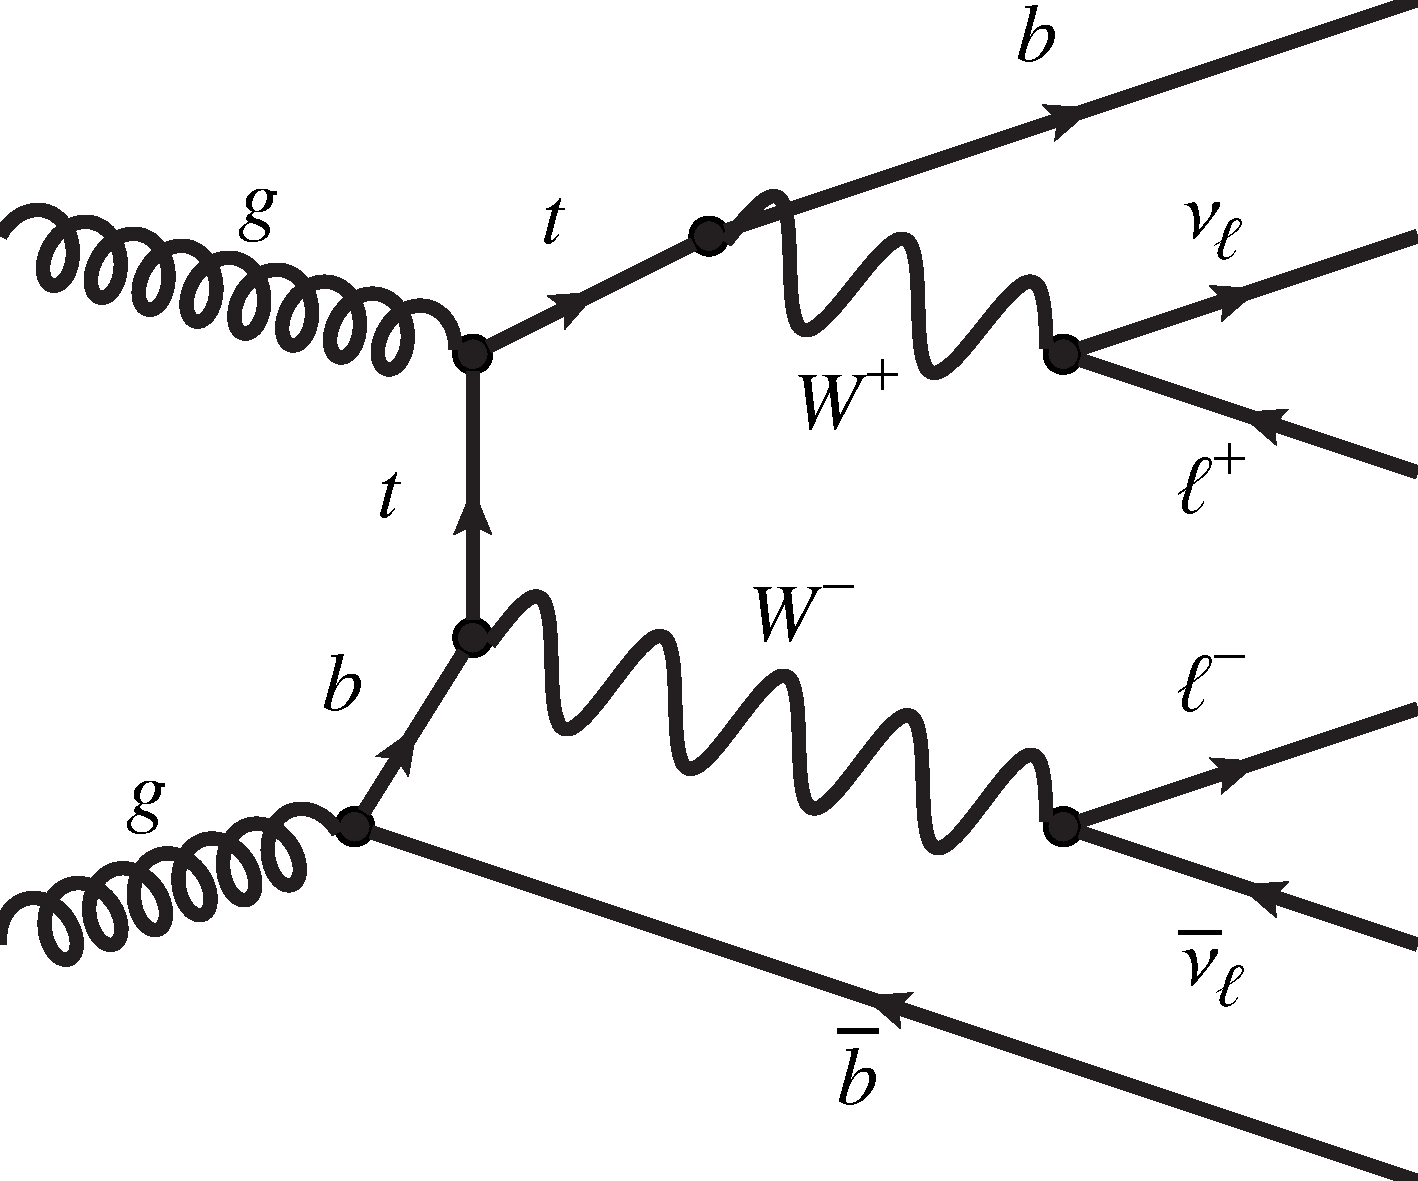
\includegraphics[width=\textwidth]{tw-NLO}
        \caption{}
        \label{fig:nlo:tw}
    \end{subfigure}
    \caption[Comparison of the final state of a \ttbar and \tW event]{Comparison of the final state of a \ttbar event~\ref{fig:nlo:ttbar} and a NLO \tW event~\ref{fig:nlo:tw}. Both \PW-bosons decay leptonically and the final states are identical.}
	\label{fig:nlo}
\end{figure}



\section{Kinematics of particle colliders}

There are a few kinematic variables and experimental properties worth discussing because they are characteristic for collider experiments which will be briefly introduced in this section.

One of the most important attributes of a collider experiment is its centre-of-mass energy, \Ecms. The centre-of-mass energy is a Lorentz invariant value which is valuable in particle physics because it denotes the available energy for particle production in an experiment.
It is defined as:
%
\begin{align}
\Ecms = \sqrt{ \left( \sum_i E_i \right)^2 - \left( \sum_i \overrightarrow{p_i} \right)^2 }
\end{align}
%
where $E_i$ and $\overrightarrow{p_i}$ are the energies and momenta of the initial or final state particles.
In the case of the Large Hadron Collider, which is simulated for the Monte Carlo samples used in this thesis and introduced in chapter \ref{chp:lhc_atlas}, two proton beams of equal energy are brought to collision resulting in an energy formula of
%
\begin{align}
\Ecms = 2 E_{beam}
\end{align}
%
assuming there are two beams with energies much higher than the particles' masses. Therefore one can neglect them in the calculation.

The second property is the instantaneous luminosity of an experiment which defines how many interactions an experiment can produce per area and time. For the colliding gaussian beams of the Large Hadron Collider it can be defined as:
%
\begin{align}
L =f \frac{n_1 n_2}{4 \pi \sigma_x \sigma_y}
\end{align}
%
where $f$ is the frequency of the beams, $n_i$ is the particle number per bunch of protons and the $\sigma_i$ values stand for the horizontal and vertical beam size respecively.
The integrated luminosity is then used to estimate the total number of interactions for a certain period of measurement:
%
\begin{align}
\mathcal{L} = \int L(t) dt
\end{align}
%
Multiplied with a cross-section the corresponding number of interactions to be expected, $N$, can be defined as $N = \sigma \mathcal{L}$.
For more information about the Standard Model and interactions in particle detectors, see ~\cite{thomson, griffiths}.

